% Created by tikzDevice version 0.12.3.1 on 2022-04-28 13:48:20
% !TEX encoding = UTF-8 Unicode
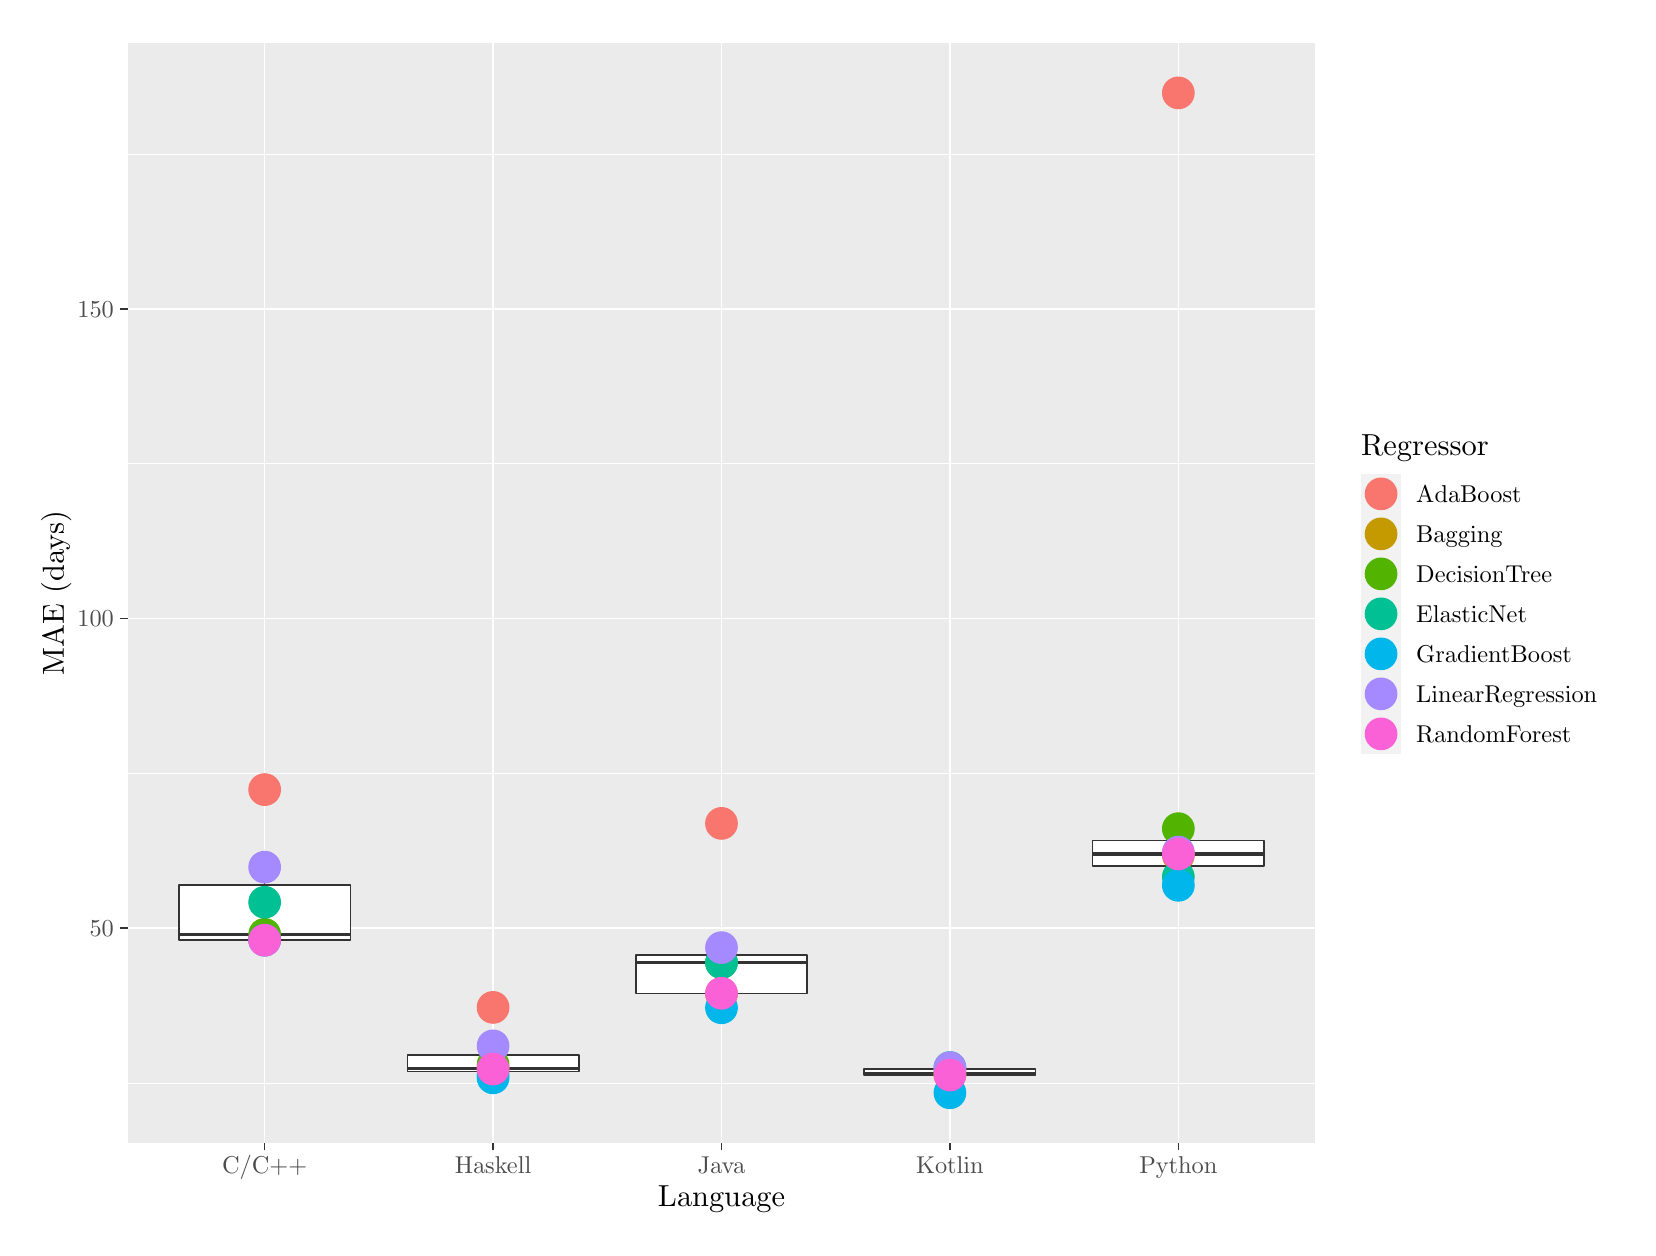
\begin{tikzpicture}[x=1pt,y=1pt]
\definecolor{fillColor}{RGB}{255,255,255}
\path[use as bounding box,fill=fillColor,fill opacity=0.00] (0,0) rectangle (578.16,433.62);
\begin{scope}
\path[clip] (  0.00,  0.00) rectangle (578.16,433.62);
\definecolor{drawColor}{RGB}{255,255,255}
\definecolor{fillColor}{RGB}{255,255,255}

\path[draw=drawColor,line width= 0.6pt,line join=round,line cap=round,fill=fillColor] (  0.00,  0.00) rectangle (578.16,433.62);
\end{scope}
\begin{scope}
\path[clip] ( 36.11, 30.69) rectangle (465.31,428.12);
\definecolor{fillColor}{gray}{0.92}

\path[fill=fillColor] ( 36.11, 30.69) rectangle (465.31,428.12);
\definecolor{drawColor}{RGB}{255,255,255}

\path[draw=drawColor,line width= 0.3pt,line join=round] ( 36.11, 52.26) --
	(465.31, 52.26);

\path[draw=drawColor,line width= 0.3pt,line join=round] ( 36.11,164.16) --
	(465.31,164.16);

\path[draw=drawColor,line width= 0.3pt,line join=round] ( 36.11,276.05) --
	(465.31,276.05);

\path[draw=drawColor,line width= 0.3pt,line join=round] ( 36.11,387.95) --
	(465.31,387.95);

\path[draw=drawColor,line width= 0.6pt,line join=round] ( 36.11,108.21) --
	(465.31,108.21);

\path[draw=drawColor,line width= 0.6pt,line join=round] ( 36.11,220.10) --
	(465.31,220.10);

\path[draw=drawColor,line width= 0.6pt,line join=round] ( 36.11,332.00) --
	(465.31,332.00);

\path[draw=drawColor,line width= 0.6pt,line join=round] ( 85.63, 30.69) --
	( 85.63,428.12);

\path[draw=drawColor,line width= 0.6pt,line join=round] (168.17, 30.69) --
	(168.17,428.12);

\path[draw=drawColor,line width= 0.6pt,line join=round] (250.71, 30.69) --
	(250.71,428.12);

\path[draw=drawColor,line width= 0.6pt,line join=round] (333.25, 30.69) --
	(333.25,428.12);

\path[draw=drawColor,line width= 0.6pt,line join=round] (415.79, 30.69) --
	(415.79,428.12);
\definecolor{drawColor}{gray}{0.20}
\definecolor{fillColor}{gray}{0.20}

\path[draw=drawColor,line width= 0.4pt,line join=round,line cap=round,fill=fillColor] ( 85.63,158.30) circle (  1.96);

\path[draw=drawColor,line width= 0.6pt,line join=round] ( 85.63,123.93) -- ( 85.63,130.28);

\path[draw=drawColor,line width= 0.6pt,line join=round] ( 85.63,104.01) -- ( 85.63,103.87);
\definecolor{fillColor}{RGB}{255,255,255}

\path[draw=drawColor,line width= 0.6pt,line join=round,line cap=round,fill=fillColor] ( 54.68,123.93) --
	( 54.68,104.01) --
	(116.59,104.01) --
	(116.59,123.93) --
	( 54.68,123.93) --
	cycle;

\path[draw=drawColor,line width= 1.1pt,line join=round] ( 54.68,105.99) -- (116.59,105.99);
\definecolor{fillColor}{gray}{0.20}

\path[draw=drawColor,line width= 0.4pt,line join=round,line cap=round,fill=fillColor] (168.17, 79.59) circle (  1.96);

\path[draw=drawColor,line width= 0.6pt,line join=round] (168.17, 62.31) -- (168.17, 65.70);

\path[draw=drawColor,line width= 0.6pt,line join=round] (168.17, 56.43) -- (168.17, 54.15);
\definecolor{fillColor}{RGB}{255,255,255}

\path[draw=drawColor,line width= 0.6pt,line join=round,line cap=round,fill=fillColor] (137.22, 62.31) --
	(137.22, 56.43) --
	(199.12, 56.43) --
	(199.12, 62.31) --
	(137.22, 62.31) --
	cycle;

\path[draw=drawColor,line width= 1.1pt,line join=round] (137.22, 57.53) -- (199.12, 57.53);
\definecolor{fillColor}{gray}{0.20}

\path[draw=drawColor,line width= 0.4pt,line join=round,line cap=round,fill=fillColor] (250.71,146.08) circle (  1.96);

\path[draw=drawColor,line width= 0.6pt,line join=round] (250.71, 98.49) -- (250.71,101.19);

\path[draw=drawColor,line width= 0.6pt,line join=round] (250.71, 84.61) -- (250.71, 79.47);
\definecolor{fillColor}{RGB}{255,255,255}

\path[draw=drawColor,line width= 0.6pt,line join=round,line cap=round,fill=fillColor] (219.76, 98.49) --
	(219.76, 84.61) --
	(281.66, 84.61) --
	(281.66, 98.49) --
	(219.76, 98.49) --
	cycle;

\path[draw=drawColor,line width= 1.1pt,line join=round] (219.76, 95.78) -- (281.66, 95.78);
\definecolor{fillColor}{gray}{0.20}

\path[draw=drawColor,line width= 0.4pt,line join=round,line cap=round,fill=fillColor] (333.25, 48.75) circle (  1.96);

\path[draw=drawColor,line width= 0.6pt,line join=round] (333.25, 57.36) -- (333.25, 57.85);

\path[draw=drawColor,line width= 0.6pt,line join=round] (333.25, 55.22) -- (333.25, 55.15);
\definecolor{fillColor}{RGB}{255,255,255}

\path[draw=drawColor,line width= 0.6pt,line join=round,line cap=round,fill=fillColor] (302.30, 57.36) --
	(302.30, 55.22) --
	(364.20, 55.22) --
	(364.20, 57.36) --
	(302.30, 57.36) --
	cycle;

\path[draw=drawColor,line width= 1.1pt,line join=round] (302.30, 55.59) -- (364.20, 55.59);
\definecolor{fillColor}{gray}{0.20}

\path[draw=drawColor,line width= 0.4pt,line join=round,line cap=round,fill=fillColor] (415.79,410.05) circle (  1.96);

\path[draw=drawColor,line width= 0.6pt,line join=round] (415.79,139.95) -- (415.79,144.18);

\path[draw=drawColor,line width= 0.6pt,line join=round] (415.79,130.64) -- (415.79,123.72);
\definecolor{fillColor}{RGB}{255,255,255}

\path[draw=drawColor,line width= 0.6pt,line join=round,line cap=round,fill=fillColor] (384.83,139.95) --
	(384.83,130.64) --
	(446.74,130.64) --
	(446.74,139.95) --
	(384.83,139.95) --
	cycle;

\path[draw=drawColor,line width= 1.1pt,line join=round] (384.83,135.03) -- (446.74,135.03);
\definecolor{drawColor}{RGB}{248,118,109}
\definecolor{fillColor}{RGB}{248,118,109}

\path[draw=drawColor,line width= 0.4pt,line join=round,line cap=round,fill=fillColor] ( 85.63,158.30) circle (  5.71);
\definecolor{drawColor}{RGB}{196,154,0}
\definecolor{fillColor}{RGB}{196,154,0}

\path[draw=drawColor,line width= 0.4pt,line join=round,line cap=round,fill=fillColor] ( 85.63,104.14) circle (  5.71);
\definecolor{drawColor}{RGB}{83,180,0}
\definecolor{fillColor}{RGB}{83,180,0}

\path[draw=drawColor,line width= 0.4pt,line join=round,line cap=round,fill=fillColor] ( 85.63,105.99) circle (  5.71);
\definecolor{drawColor}{RGB}{0,192,148}
\definecolor{fillColor}{RGB}{0,192,148}

\path[draw=drawColor,line width= 0.4pt,line join=round,line cap=round,fill=fillColor] ( 85.63,117.58) circle (  5.71);
\definecolor{drawColor}{RGB}{0,182,235}
\definecolor{fillColor}{RGB}{0,182,235}

\path[draw=drawColor,line width= 0.4pt,line join=round,line cap=round,fill=fillColor] ( 85.63,103.88) circle (  5.71);
\definecolor{drawColor}{RGB}{165,138,255}
\definecolor{fillColor}{RGB}{165,138,255}

\path[draw=drawColor,line width= 0.4pt,line join=round,line cap=round,fill=fillColor] ( 85.63,130.28) circle (  5.71);
\definecolor{drawColor}{RGB}{251,97,215}
\definecolor{fillColor}{RGB}{251,97,215}

\path[draw=drawColor,line width= 0.4pt,line join=round,line cap=round,fill=fillColor] ( 85.63,103.87) circle (  5.71);
\definecolor{drawColor}{RGB}{248,118,109}
\definecolor{fillColor}{RGB}{248,118,109}

\path[draw=drawColor,line width= 0.4pt,line join=round,line cap=round,fill=fillColor] (168.17, 79.59) circle (  5.71);
\definecolor{drawColor}{RGB}{196,154,0}
\definecolor{fillColor}{RGB}{196,154,0}

\path[draw=drawColor,line width= 0.4pt,line join=round,line cap=round,fill=fillColor] (168.17, 57.53) circle (  5.71);
\definecolor{drawColor}{RGB}{83,180,0}
\definecolor{fillColor}{RGB}{83,180,0}

\path[draw=drawColor,line width= 0.4pt,line join=round,line cap=round,fill=fillColor] (168.17, 58.91) circle (  5.71);
\definecolor{drawColor}{RGB}{0,192,148}
\definecolor{fillColor}{RGB}{0,192,148}

\path[draw=drawColor,line width= 0.4pt,line join=round,line cap=round,fill=fillColor] (168.17, 55.55) circle (  5.71);
\definecolor{drawColor}{RGB}{0,182,235}
\definecolor{fillColor}{RGB}{0,182,235}

\path[draw=drawColor,line width= 0.4pt,line join=round,line cap=round,fill=fillColor] (168.17, 54.15) circle (  5.71);
\definecolor{drawColor}{RGB}{165,138,255}
\definecolor{fillColor}{RGB}{165,138,255}

\path[draw=drawColor,line width= 0.4pt,line join=round,line cap=round,fill=fillColor] (168.17, 65.70) circle (  5.71);
\definecolor{drawColor}{RGB}{251,97,215}
\definecolor{fillColor}{RGB}{251,97,215}

\path[draw=drawColor,line width= 0.4pt,line join=round,line cap=round,fill=fillColor] (168.17, 57.31) circle (  5.71);
\definecolor{drawColor}{RGB}{248,118,109}
\definecolor{fillColor}{RGB}{248,118,109}

\path[draw=drawColor,line width= 0.4pt,line join=round,line cap=round,fill=fillColor] (250.71,146.08) circle (  5.71);
\definecolor{drawColor}{RGB}{196,154,0}
\definecolor{fillColor}{RGB}{196,154,0}

\path[draw=drawColor,line width= 0.4pt,line join=round,line cap=round,fill=fillColor] (250.71, 84.52) circle (  5.71);
\definecolor{drawColor}{RGB}{83,180,0}
\definecolor{fillColor}{RGB}{83,180,0}

\path[draw=drawColor,line width= 0.4pt,line join=round,line cap=round,fill=fillColor] (250.71, 95.79) circle (  5.71);
\definecolor{drawColor}{RGB}{0,192,148}
\definecolor{fillColor}{RGB}{0,192,148}

\path[draw=drawColor,line width= 0.4pt,line join=round,line cap=round,fill=fillColor] (250.71, 95.78) circle (  5.71);
\definecolor{drawColor}{RGB}{0,182,235}
\definecolor{fillColor}{RGB}{0,182,235}

\path[draw=drawColor,line width= 0.4pt,line join=round,line cap=round,fill=fillColor] (250.71, 79.47) circle (  5.71);
\definecolor{drawColor}{RGB}{165,138,255}
\definecolor{fillColor}{RGB}{165,138,255}

\path[draw=drawColor,line width= 0.4pt,line join=round,line cap=round,fill=fillColor] (250.71,101.19) circle (  5.71);
\definecolor{drawColor}{RGB}{251,97,215}
\definecolor{fillColor}{RGB}{251,97,215}

\path[draw=drawColor,line width= 0.4pt,line join=round,line cap=round,fill=fillColor] (250.71, 84.70) circle (  5.71);
\definecolor{drawColor}{RGB}{248,118,109}
\definecolor{fillColor}{RGB}{248,118,109}

\path[draw=drawColor,line width= 0.4pt,line join=round,line cap=round,fill=fillColor] (333.25, 56.89) circle (  5.71);
\definecolor{drawColor}{RGB}{196,154,0}
\definecolor{fillColor}{RGB}{196,154,0}

\path[draw=drawColor,line width= 0.4pt,line join=round,line cap=round,fill=fillColor] (333.25, 55.30) circle (  5.71);
\definecolor{drawColor}{RGB}{83,180,0}
\definecolor{fillColor}{RGB}{83,180,0}

\path[draw=drawColor,line width= 0.4pt,line join=round,line cap=round,fill=fillColor] (333.25, 55.59) circle (  5.71);
\definecolor{drawColor}{RGB}{0,192,148}
\definecolor{fillColor}{RGB}{0,192,148}

\path[draw=drawColor,line width= 0.4pt,line join=round,line cap=round,fill=fillColor] (333.25, 57.85) circle (  5.71);
\definecolor{drawColor}{RGB}{0,182,235}
\definecolor{fillColor}{RGB}{0,182,235}

\path[draw=drawColor,line width= 0.4pt,line join=round,line cap=round,fill=fillColor] (333.25, 48.75) circle (  5.71);
\definecolor{drawColor}{RGB}{165,138,255}
\definecolor{fillColor}{RGB}{165,138,255}

\path[draw=drawColor,line width= 0.4pt,line join=round,line cap=round,fill=fillColor] (333.25, 57.83) circle (  5.71);
\definecolor{drawColor}{RGB}{251,97,215}
\definecolor{fillColor}{RGB}{251,97,215}

\path[draw=drawColor,line width= 0.4pt,line join=round,line cap=round,fill=fillColor] (333.25, 55.15) circle (  5.71);
\definecolor{drawColor}{RGB}{248,118,109}
\definecolor{fillColor}{RGB}{248,118,109}

\path[draw=drawColor,line width= 0.4pt,line join=round,line cap=round,fill=fillColor] (415.79,410.05) circle (  5.71);
\definecolor{drawColor}{RGB}{196,154,0}
\definecolor{fillColor}{RGB}{196,154,0}

\path[draw=drawColor,line width= 0.4pt,line join=round,line cap=round,fill=fillColor] (415.79,134.53) circle (  5.71);
\definecolor{drawColor}{RGB}{83,180,0}
\definecolor{fillColor}{RGB}{83,180,0}

\path[draw=drawColor,line width= 0.4pt,line join=round,line cap=round,fill=fillColor] (415.79,144.18) circle (  5.71);
\definecolor{drawColor}{RGB}{0,192,148}
\definecolor{fillColor}{RGB}{0,192,148}

\path[draw=drawColor,line width= 0.4pt,line join=round,line cap=round,fill=fillColor] (415.79,126.76) circle (  5.71);
\definecolor{drawColor}{RGB}{0,182,235}
\definecolor{fillColor}{RGB}{0,182,235}

\path[draw=drawColor,line width= 0.4pt,line join=round,line cap=round,fill=fillColor] (415.79,123.72) circle (  5.71);
\definecolor{drawColor}{RGB}{165,138,255}
\definecolor{fillColor}{RGB}{165,138,255}

\path[draw=drawColor,line width= 0.4pt,line join=round,line cap=round,fill=fillColor] (415.79,135.71) circle (  5.71);
\definecolor{drawColor}{RGB}{251,97,215}
\definecolor{fillColor}{RGB}{251,97,215}

\path[draw=drawColor,line width= 0.4pt,line join=round,line cap=round,fill=fillColor] (415.79,135.03) circle (  5.71);
\end{scope}
\begin{scope}
\path[clip] (  0.00,  0.00) rectangle (578.16,433.62);
\definecolor{drawColor}{gray}{0.30}

\node[text=drawColor,anchor=base east,inner sep=0pt, outer sep=0pt, scale=  0.88] at ( 31.16,105.18) {50};

\node[text=drawColor,anchor=base east,inner sep=0pt, outer sep=0pt, scale=  0.88] at ( 31.16,217.07) {100};

\node[text=drawColor,anchor=base east,inner sep=0pt, outer sep=0pt, scale=  0.88] at ( 31.16,328.97) {150};
\end{scope}
\begin{scope}
\path[clip] (  0.00,  0.00) rectangle (578.16,433.62);
\definecolor{drawColor}{gray}{0.20}

\path[draw=drawColor,line width= 0.6pt,line join=round] ( 33.36,108.21) --
	( 36.11,108.21);

\path[draw=drawColor,line width= 0.6pt,line join=round] ( 33.36,220.10) --
	( 36.11,220.10);

\path[draw=drawColor,line width= 0.6pt,line join=round] ( 33.36,332.00) --
	( 36.11,332.00);
\end{scope}
\begin{scope}
\path[clip] (  0.00,  0.00) rectangle (578.16,433.62);
\definecolor{drawColor}{gray}{0.20}

\path[draw=drawColor,line width= 0.6pt,line join=round] ( 85.63, 27.94) --
	( 85.63, 30.69);

\path[draw=drawColor,line width= 0.6pt,line join=round] (168.17, 27.94) --
	(168.17, 30.69);

\path[draw=drawColor,line width= 0.6pt,line join=round] (250.71, 27.94) --
	(250.71, 30.69);

\path[draw=drawColor,line width= 0.6pt,line join=round] (333.25, 27.94) --
	(333.25, 30.69);

\path[draw=drawColor,line width= 0.6pt,line join=round] (415.79, 27.94) --
	(415.79, 30.69);
\end{scope}
\begin{scope}
\path[clip] (  0.00,  0.00) rectangle (578.16,433.62);
\definecolor{drawColor}{gray}{0.30}

\node[text=drawColor,anchor=base,inner sep=0pt, outer sep=0pt, scale=  0.88] at ( 85.63, 19.68) {C/C++};

\node[text=drawColor,anchor=base,inner sep=0pt, outer sep=0pt, scale=  0.88] at (168.17, 19.68) {Haskell};

\node[text=drawColor,anchor=base,inner sep=0pt, outer sep=0pt, scale=  0.88] at (250.71, 19.68) {Java};

\node[text=drawColor,anchor=base,inner sep=0pt, outer sep=0pt, scale=  0.88] at (333.25, 19.68) {Kotlin};

\node[text=drawColor,anchor=base,inner sep=0pt, outer sep=0pt, scale=  0.88] at (415.79, 19.68) {Python};
\end{scope}
\begin{scope}
\path[clip] (  0.00,  0.00) rectangle (578.16,433.62);
\definecolor{drawColor}{RGB}{0,0,0}

\node[text=drawColor,anchor=base,inner sep=0pt, outer sep=0pt, scale=  1.10] at (250.71,  7.64) {Language};
\end{scope}
\begin{scope}
\path[clip] (  0.00,  0.00) rectangle (578.16,433.62);
\definecolor{drawColor}{RGB}{0,0,0}

\node[text=drawColor,rotate= 90.00,anchor=base,inner sep=0pt, outer sep=0pt, scale=  1.10] at ( 13.08,229.40) {MAE (days)};
\end{scope}
\begin{scope}
\path[clip] (  0.00,  0.00) rectangle (578.16,433.62);
\definecolor{fillColor}{RGB}{255,255,255}

\path[fill=fillColor] (476.31,165.71) rectangle (572.66,293.10);
\end{scope}
\begin{scope}
\path[clip] (  0.00,  0.00) rectangle (578.16,433.62);
\definecolor{drawColor}{RGB}{0,0,0}

\node[text=drawColor,anchor=base west,inner sep=0pt, outer sep=0pt, scale=  1.10] at (481.81,278.95) {Regressor};
\end{scope}
\begin{scope}
\path[clip] (  0.00,  0.00) rectangle (578.16,433.62);
\definecolor{fillColor}{gray}{0.95}

\path[fill=fillColor] (481.81,257.93) rectangle (496.26,272.38);
\end{scope}
\begin{scope}
\path[clip] (  0.00,  0.00) rectangle (578.16,433.62);
\definecolor{drawColor}{RGB}{248,118,109}
\definecolor{fillColor}{RGB}{248,118,109}

\path[draw=drawColor,line width= 0.4pt,line join=round,line cap=round,fill=fillColor] (489.04,265.16) circle (  5.71);
\end{scope}
\begin{scope}
\path[clip] (  0.00,  0.00) rectangle (578.16,433.62);
\definecolor{fillColor}{gray}{0.95}

\path[fill=fillColor] (481.81,243.48) rectangle (496.26,257.93);
\end{scope}
\begin{scope}
\path[clip] (  0.00,  0.00) rectangle (578.16,433.62);
\definecolor{drawColor}{RGB}{196,154,0}
\definecolor{fillColor}{RGB}{196,154,0}

\path[draw=drawColor,line width= 0.4pt,line join=round,line cap=round,fill=fillColor] (489.04,250.70) circle (  5.71);
\end{scope}
\begin{scope}
\path[clip] (  0.00,  0.00) rectangle (578.16,433.62);
\definecolor{fillColor}{gray}{0.95}

\path[fill=fillColor] (481.81,229.02) rectangle (496.26,243.48);
\end{scope}
\begin{scope}
\path[clip] (  0.00,  0.00) rectangle (578.16,433.62);
\definecolor{drawColor}{RGB}{83,180,0}
\definecolor{fillColor}{RGB}{83,180,0}

\path[draw=drawColor,line width= 0.4pt,line join=round,line cap=round,fill=fillColor] (489.04,236.25) circle (  5.71);
\end{scope}
\begin{scope}
\path[clip] (  0.00,  0.00) rectangle (578.16,433.62);
\definecolor{fillColor}{gray}{0.95}

\path[fill=fillColor] (481.81,214.57) rectangle (496.26,229.02);
\end{scope}
\begin{scope}
\path[clip] (  0.00,  0.00) rectangle (578.16,433.62);
\definecolor{drawColor}{RGB}{0,192,148}
\definecolor{fillColor}{RGB}{0,192,148}

\path[draw=drawColor,line width= 0.4pt,line join=round,line cap=round,fill=fillColor] (489.04,221.80) circle (  5.71);
\end{scope}
\begin{scope}
\path[clip] (  0.00,  0.00) rectangle (578.16,433.62);
\definecolor{fillColor}{gray}{0.95}

\path[fill=fillColor] (481.81,200.11) rectangle (496.26,214.57);
\end{scope}
\begin{scope}
\path[clip] (  0.00,  0.00) rectangle (578.16,433.62);
\definecolor{drawColor}{RGB}{0,182,235}
\definecolor{fillColor}{RGB}{0,182,235}

\path[draw=drawColor,line width= 0.4pt,line join=round,line cap=round,fill=fillColor] (489.04,207.34) circle (  5.71);
\end{scope}
\begin{scope}
\path[clip] (  0.00,  0.00) rectangle (578.16,433.62);
\definecolor{fillColor}{gray}{0.95}

\path[fill=fillColor] (481.81,185.66) rectangle (496.26,200.11);
\end{scope}
\begin{scope}
\path[clip] (  0.00,  0.00) rectangle (578.16,433.62);
\definecolor{drawColor}{RGB}{165,138,255}
\definecolor{fillColor}{RGB}{165,138,255}

\path[draw=drawColor,line width= 0.4pt,line join=round,line cap=round,fill=fillColor] (489.04,192.89) circle (  5.71);
\end{scope}
\begin{scope}
\path[clip] (  0.00,  0.00) rectangle (578.16,433.62);
\definecolor{fillColor}{gray}{0.95}

\path[fill=fillColor] (481.81,171.21) rectangle (496.26,185.66);
\end{scope}
\begin{scope}
\path[clip] (  0.00,  0.00) rectangle (578.16,433.62);
\definecolor{drawColor}{RGB}{251,97,215}
\definecolor{fillColor}{RGB}{251,97,215}

\path[draw=drawColor,line width= 0.4pt,line join=round,line cap=round,fill=fillColor] (489.04,178.43) circle (  5.71);
\end{scope}
\begin{scope}
\path[clip] (  0.00,  0.00) rectangle (578.16,433.62);
\definecolor{drawColor}{RGB}{0,0,0}

\node[text=drawColor,anchor=base west,inner sep=0pt, outer sep=0pt, scale=  0.88] at (501.76,262.13) {AdaBoost};
\end{scope}
\begin{scope}
\path[clip] (  0.00,  0.00) rectangle (578.16,433.62);
\definecolor{drawColor}{RGB}{0,0,0}

\node[text=drawColor,anchor=base west,inner sep=0pt, outer sep=0pt, scale=  0.88] at (501.76,247.67) {Bagging};
\end{scope}
\begin{scope}
\path[clip] (  0.00,  0.00) rectangle (578.16,433.62);
\definecolor{drawColor}{RGB}{0,0,0}

\node[text=drawColor,anchor=base west,inner sep=0pt, outer sep=0pt, scale=  0.88] at (501.76,233.22) {DecisionTree};
\end{scope}
\begin{scope}
\path[clip] (  0.00,  0.00) rectangle (578.16,433.62);
\definecolor{drawColor}{RGB}{0,0,0}

\node[text=drawColor,anchor=base west,inner sep=0pt, outer sep=0pt, scale=  0.88] at (501.76,218.77) {ElasticNet};
\end{scope}
\begin{scope}
\path[clip] (  0.00,  0.00) rectangle (578.16,433.62);
\definecolor{drawColor}{RGB}{0,0,0}

\node[text=drawColor,anchor=base west,inner sep=0pt, outer sep=0pt, scale=  0.88] at (501.76,204.31) {GradientBoost};
\end{scope}
\begin{scope}
\path[clip] (  0.00,  0.00) rectangle (578.16,433.62);
\definecolor{drawColor}{RGB}{0,0,0}

\node[text=drawColor,anchor=base west,inner sep=0pt, outer sep=0pt, scale=  0.88] at (501.76,189.86) {LinearRegression};
\end{scope}
\begin{scope}
\path[clip] (  0.00,  0.00) rectangle (578.16,433.62);
\definecolor{drawColor}{RGB}{0,0,0}

\node[text=drawColor,anchor=base west,inner sep=0pt, outer sep=0pt, scale=  0.88] at (501.76,175.40) {RandomForest};
\end{scope}
\end{tikzpicture}
